
Dans ce chapitre est présenté le robot humanoïde Sigmaban sur 
lequel s'appuie ces travaux.
Tout d'abord les aspects matériels avec la description de la plateforme 
sont abordés, ainsi que les différents défauts motivant les travaux de cette thèse. 
Deuxièmement la modélisation géométrique de cette plateforme est décrite. 
Enfin le mouvement de marche sur qui repose les expérimentations de l'odométrie 
est présenté.

\section{La plateforme robotique Sigmaban\label{sec:robot}}

Le robot Sigmaban est conçu, développé et fabriqué 
par les membres de l'équipe Rhoban depuis 2011.
L'objet même de ce robot est la participation aux matchs 
de football robotique de la compétition internationale RoboCup ; et 
plus précisément dans la ligue des petits 
robots humanoïde \textit{Kid-Size}.
Les sections ci dessous présentent un historique rapide
de l'évolution de la plateforme, une description
de ses composants dans sa version 2017 puis énumèrent
les sources d'imperfections du robot.

\subsection{Évolution de la plateforme}

\begin{figure}[htb]
    \centerfloat
    \begin{subfigure}{0.3\paperwidth}
        \centering
        \includegraphics[width=0.7\linewidth]{../media/acroban.jpg}
    \end{subfigure}
    \begin{subfigure}{0.3\paperwidth}
        \centering
        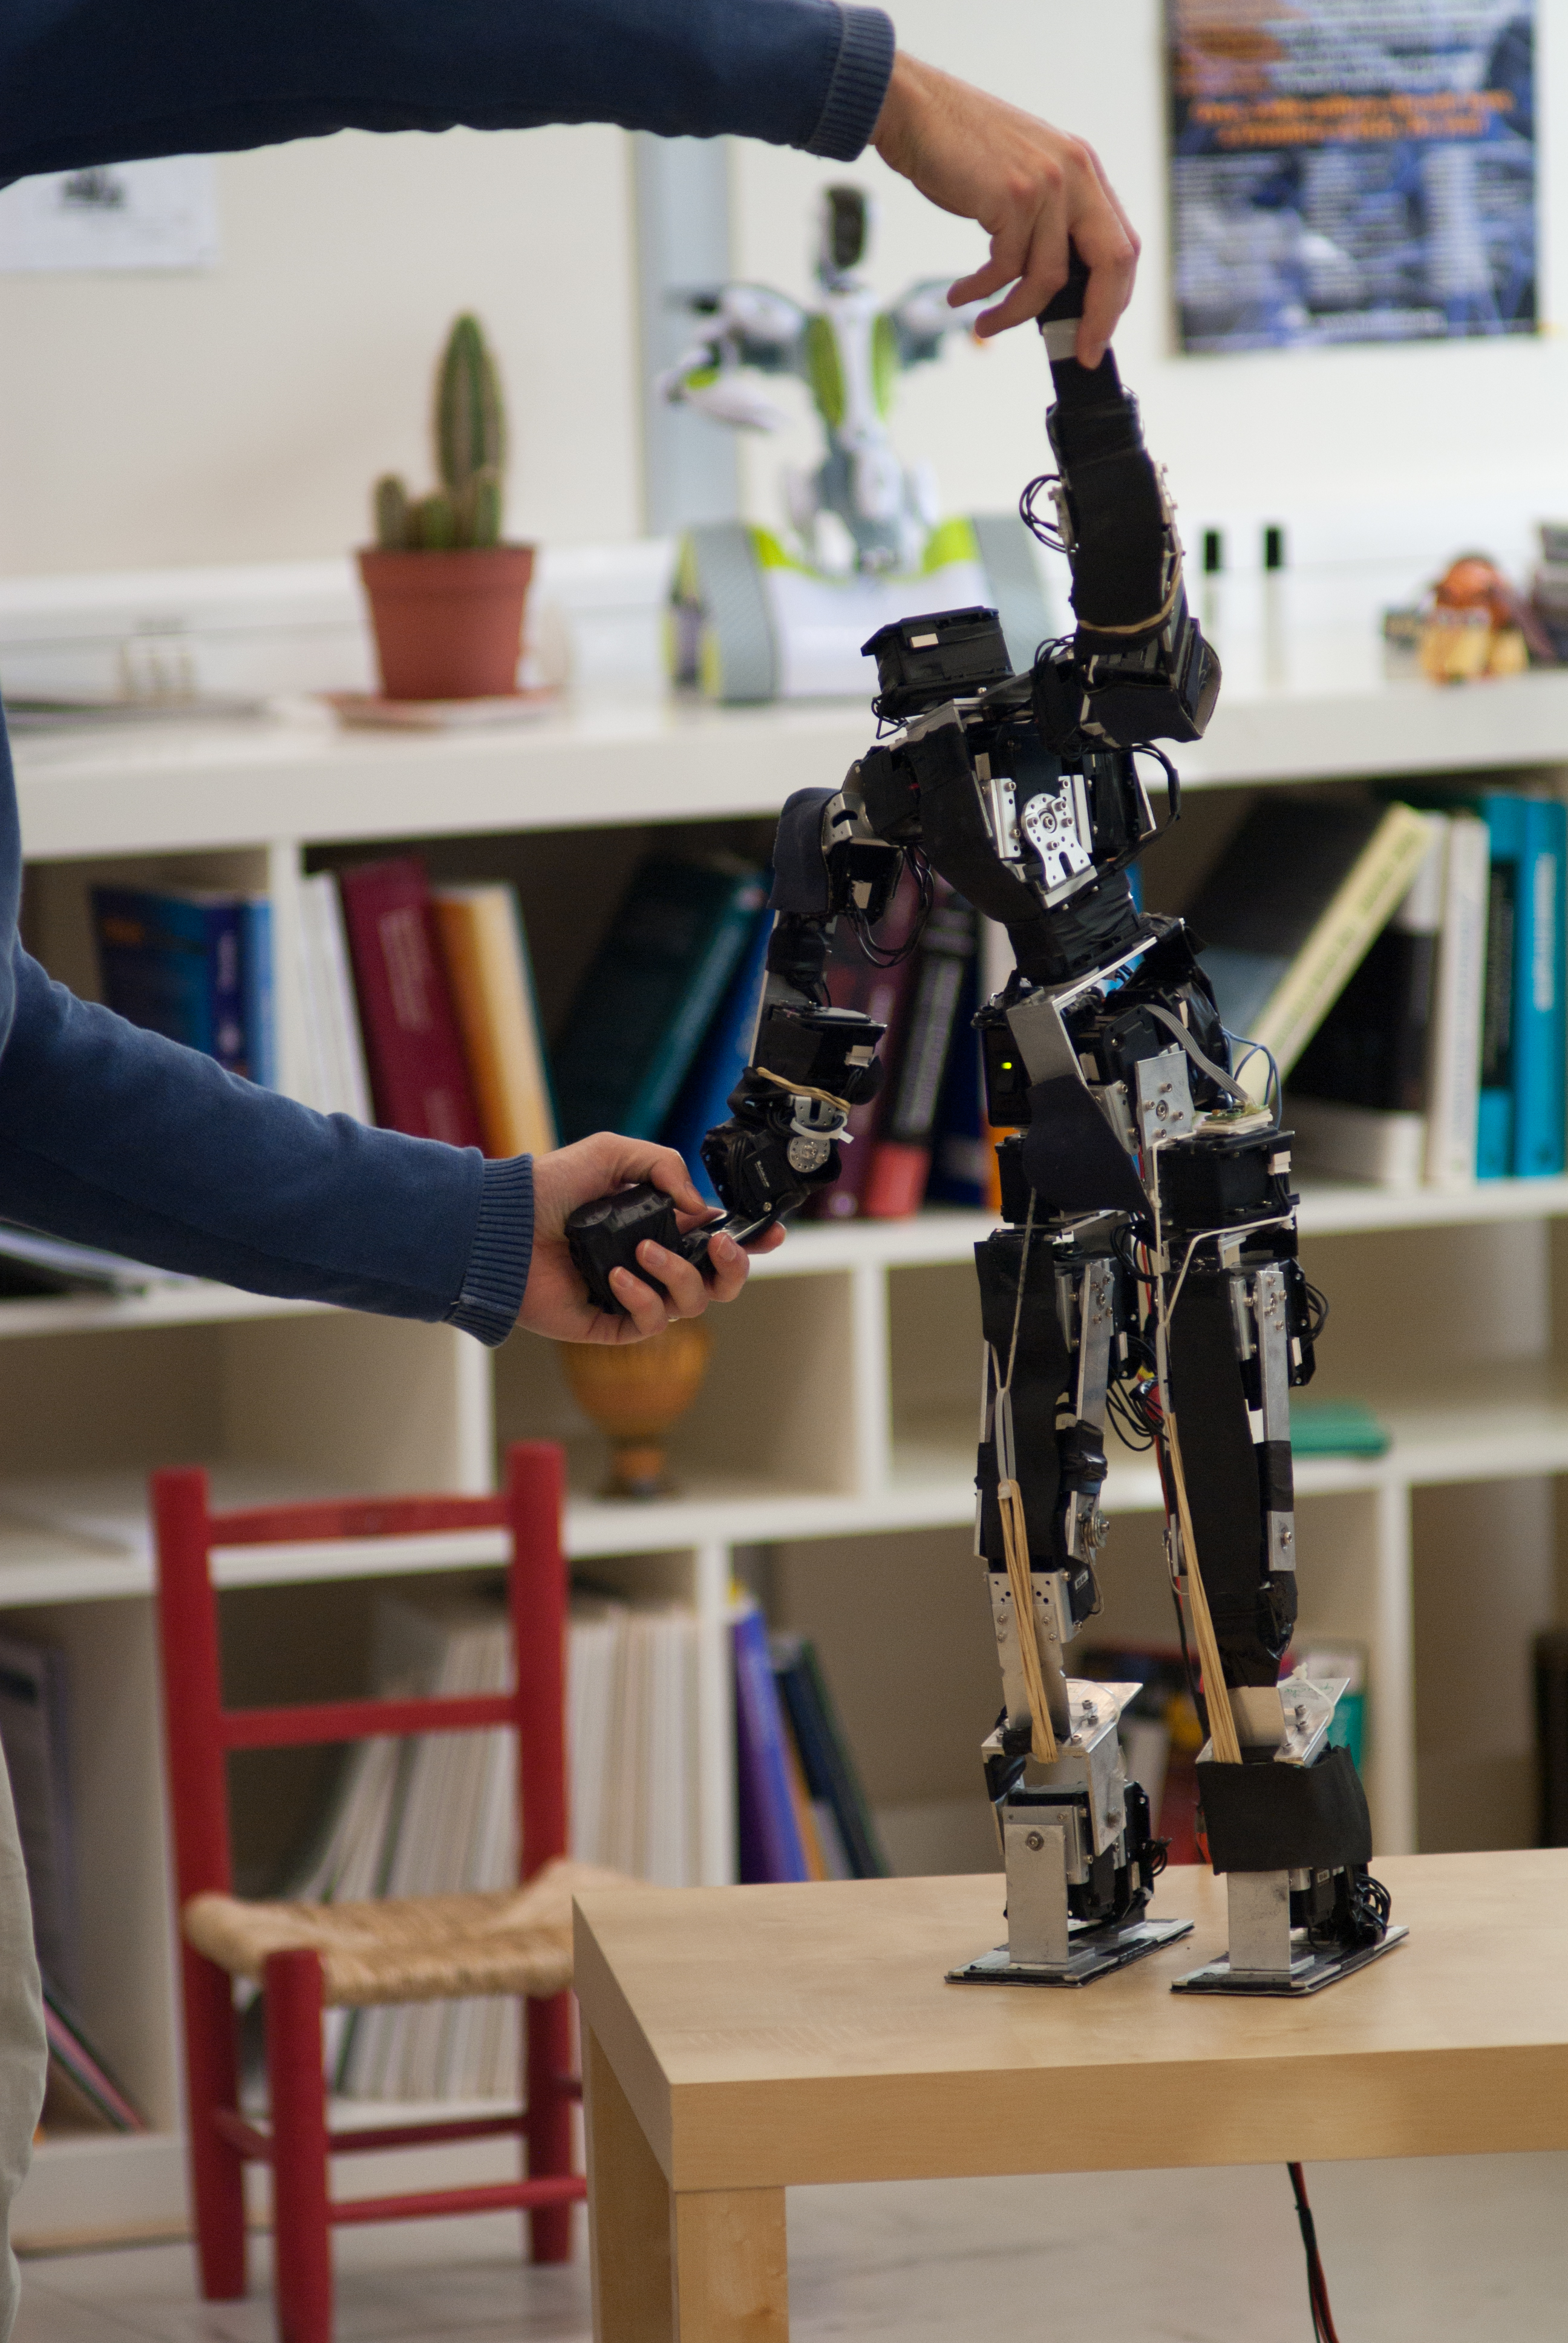
\includegraphics[width=0.9\linewidth]{../media/acroban2.jpg}
    \end{subfigure}
    \caption{\label{fig:robot_acroban} 
        Le robot Acroban, ancêtre de Sigmaban.
    }
\end{figure}

Le robot humanoïde Acroban, représenté sur la 
figure \ref{fig:robot_acroban}, est l'un des premiers robots 
conçus et construits par l'équipe Rhoban utilisant 
les servomoteurs Dynamixel.
Il peut être considéré comme l'ancêtre du robot Sigmaban.
Plus grand que Sigmaban, Acroban possède également plus de degrés de liberté, 
soit $26$ articulations. 
Ce robot à servi de plateforme expérimentale dans l'équipe 
\textit{FLOWERS} de l'INRIA 
(\cite{ly_acroban_2010}, \cite{lapeyre_maturational_2011},
\cite{ly_bio-inspired_2011}, \cite{oudeyer_exploring_2011}).
Des domaines variés comme l'interaction homme-robot, 
la \textit{compliance}\footnote{Mouvement souple, s'adaptant 
activement ou passivement au contact avec l'environnement.}
des mouvements (par exemple de la colonne vertébrale),
la robotique développementale ont été expérimentés.
Ce robot a de plus été utile à l'équipe pour appréhender les problématiques
posées par la mécatronique, les moteurs, le contrôle 
et la programmation des robots humanoïdes.
La locomotion de ce robot était fonctionnelle bien que peu rapide
en comparaison de sa taille.\\

\begin{figure}[htb]
    \centerfloat
    \begin{subfigure}{0.3\paperwidth}
        \centering
        \includegraphics[width=0.9\linewidth]{../media/sigmaban_1_0.jpg}
    \end{subfigure}
    \begin{subfigure}{0.3\paperwidth}
        \centering
        \includegraphics[width=0.9\linewidth]{../media/sigmaban_1_1.jpg}
    \end{subfigure}
    \begin{subfigure}{0.3\paperwidth}
        \centering
        \includegraphics[width=0.84\linewidth]{../media/sigmaban_1_2_crop.jpg}
    \end{subfigure}
    \newline
    \begin{subfigure}{0.3\paperwidth}
        \centering
        \includegraphics[angle=-90,width=0.9\linewidth]{../media/sigmaban_1_3.jpg}
    \end{subfigure}
    \begin{subfigure}{0.3\paperwidth}
        \centering
        \includegraphics[angle=-90,width=0.9\linewidth]{../media/sigmaban_1_4.jpg}
    \end{subfigure}
    \begin{subfigure}{0.3\paperwidth}
        \centering
        \includegraphics[width=0.915\linewidth]{../media/sigmaban_1_5_crop.jpg}
    \end{subfigure}
    \caption{\label{fig:robot_sigmaban_evolution} 
        Évolution du robot Sigmaban de gauche à droite et de haut en bas de 2011 à 2016.
    }
\end{figure}

De 2011 à 2017, la plateforme Sigmaban n'a pas cessé d'évoluer.
Son développement étant rythmé par la participation chaque année 
à la compétition RoboCup.
La figure \ref{fig:robot_sigmaban_evolution} retrace cette évolution et montre
l'apparence du robot année après année.
Les principales étapes de cette évolution dont j'ai été témoin et 
quelques fois acteur sont les suivantes :
\begin{itemize}
    \item Les premières versions de Sigmaban comportaient $22$ servomoteurs.
        Comme chez Acroban, deux articulations étaient présentes dans le dos
        du robot au dessus du bassin. 
        De plus, des amortisseurs (soit un degré de liberté non contrôlé) étaient 
        fixés au niveau des hanches du robot.
        Malgré l'intérêt de ces innovations mécaniques, elles ont été
        retirées en 2014 pour venir vers l'architecture mécanique \og classique \fg
        des robots humanoïde de la RoboCup avec $20$ servomoteurs.
        En raison du jeu mécanique supplémentaire induit par ces articulations, 
        cette architecture n'était pas en l'état suffisamment compétitive. 
        Sa marche était trop instable.
    \item Mise en place en 2014 d'une architecture logicielle pour le module de vision 
        basée sur un \textit{pipeline} de filtres (et \textit{OpenCV}).
        Les images de la caméra sont analysées successivement au travers d'un graphe 
        de traitements indépendants.
        Cette architecture rend le système plus facilement configurable, flexible
        et plus rapidement adaptable aux conditions visuelles d'un 
        nouvel environnement RoboCup.
    \item Entre 2014 et 2015, l'écriture du générateur de marche en boucle ouverte
        (\textit{IKWalk}) a permis d'améliorer la stabilité et la maniabilité 
        du déplacement du robot (voir section \ref{sec:walk}).
    \item Le renouvellement progressif à partir de 2015 des servomoteurs Dynamixel  
        remplace la gamme \textit{RX} par la gamme \textit{MX}.
        L'utilisation d'encodeurs magnétiques plus précis et moins sensibles 
        à l'usure mécanique que les potentiomètres améliore au fur et à mesure 
        la qualité des mouvements du robot.
    \item Le module de localisation basé sur un filtre particulaire 
        a commencé à être employé en 2015.
        Il s'appuie sur la détection des bases des poteaux de but ainsi 
        que sur les bordures du terrain pour situer le robot de manière absolue 
        lors d'un match de football robotique.
    \item Depuis 2015, les déplacements du robot sont intégrés par l'implémentation 
        d'un modèle géométrique direct (section \ref{sec:modele_direct}) 
        et de la reconstruction de l'état du robot (section \ref{sec:estimation_etat})
        à partir de ses capteurs.
        L'information de l'odométrie est particulièrement importante 
        pour le processus de localisation et d'asservissement des ordres de la marche.
    \item Le développement des capteurs de pression en 2015 sous les pieds des robots
        est concomitant à l'introduction de l'herbe artificielle comme surface de marche
        par la RoboCup.
        Pour réduire une grande partie de l'effet de déstabilisation de l'herbe artificielle, 
        des crampons sont ajoutés aux pieds des robots.
        Les capteurs de pression y sont directement attachés. 
        Ces capteurs sont essentiels à l'odométrie (section \ref{sec:odometry_pressure}) 
        et au processus de stabilisation de la marche.
    \item Une refonte de toute l'architecture logicielle a été entreprise en 2015.
        Précédemment, le programme principal contrôlant le robot comportait, à la manière 
        de \textit{ROS} (\textit{Robot Operating System}), 
        plusieurs modules indépendants et communicant par envoi de messages.
        Une interface graphique écrite en C\# permettait de contrôler et 
        de superviser les robots.
        À ceci a été préféré une architecture purement monolithique, simplifiant
        la communication des différents modules.
        Une bibliothèque de configuration, de monitorage et de contrôle du robot a été
        développée (\textit{RhIO}) avec un \textit{shell} (textuel) comme interface 
        utilisateur.
    \item En 2016, la conception d'une nouvelle carte électronique a
        séparé la communication avec les servomoteurs en trois bus séries distincts.
        Grâce également à la réimplémentation de la gestion de la communication bas niveau 
        au niveau de l'ordinateur embarqué (bibliothèque \textit{RhAL}, 
        voir section \ref{sec:other_works})
        il a été possible de doubler la fréquence de la boucle de lecture-écriture 
        de $50$~Hz à $100$~Hz.
        Cette augmentation de fréquence a amélioré la fluidité de tous les mouvements.
    \item La \textit{webcam} au niveau de la tête du robot a été remplacée en 2016
        par une caméra dite \og industrielle \fg. 
        Ces caméras ont pour principal intérêt une capture de l'image par 
        \textit{global shutter} plutôt que par \textit{rolling Shutter}.
        Tous les pixels du capteur enregistrent l'image au même moment plutôt que
        ligne par ligne.
        Ceci réduit grandement le flou dû aux mouvements de la tête du robot.
        De plus, elles sont plus finement paramétrables 
        (balance des couleurs, vitesse d'obturation, ...).
        
        En 2017, l'API propriétaire (en remplacement de \textit{v4l2}) a permis une meilleure 
        maitrise des horodatages de capture des images.
        Ce qui a amélioré la synchronisation temporelle entre la caméra 
        et les autres capteurs\footnote{Connaitre avec exactitude la valeur des capteurs 
        (encodeurs, IMU) du robot au moment de la prise d'image est crucial pour 
        la précision du calcul de la position cartésienne relative des objets détectés dans l'image. 
        La difficulté réside dans la synchronisation des horodatages
        entre les lectures bas niveau sur le bus de communication série et le pilote de la caméra.}.
        D'une connectique USB 3.0 en 2016, nous sommes passés en 2017 
        à une liaison ethernet entre la caméra et l'ordinateur embarqué
        pour des raisons d'interférences électromagnétiques entre 
        le câble USB 3.0 et la communication radio WiFi.
        Enfin, le choix personnalisé de la lentille (grand angle ou petit angle)
        laisse plus de liberté quand à la stratégie de scan et de détection
        (compromis entre l'ouverture angulaire, la résolution de l'image par degré, 
        la déformation de l'image et le temps de balayage du terrain).
    \item L'utilisation en 2017 d'un apprentissage par un réseau de neurones profond 
        pour la détection de la balle et des buts a radicalement amélioré la vision du robot.
        Les réseaux de neurones ont apporté une plus grande robustesse aux conditions lumineuses, 
        à l'occlusion partielle des objets, moins de faux positifs ainsi 
        qu'une plus grande portée de détection.
    \item Le développement d'une nouvelle marche en 2017, la \textit{QuinticWalk} toujours
        dans l'espace cartésien mais basée sur des splines polynomiales de degré $5$
        a apporté une meilleure stabilité du déplacement, particulièrement importante 
        sur le plus grand robot (voir section \ref{sec:other_works}).\\
\end{itemize}

\begin{figure}[htb]
    \centerfloat
    \begin{subfigure}{0.35\paperwidth}
        \centering
        \includegraphics[width=0.7\linewidth]{../media/grosban_1_0.jpg}
    \end{subfigure}
    \begin{subfigure}{0.35\paperwidth}
        \centering
        \includegraphics[width=1.0\linewidth]{../media/grosban_1_1.png}
    \end{subfigure}
    \caption{\label{fig:robot_grosban} 
        Le robot Grosban, une version plus grande et plus puissante de Sigmaban.
        À gauche, la première version de $90$~cm en 2015 et à droite, 
        la deuxième version plus petite à $75$~cm en 2016.
    }
\end{figure}

\begin{figure}[htb]
    \centerfloat
    \includegraphics[width=0.4\linewidth]{../media/sigmaban_1_6.png}
    \includegraphics[width=0.4\linewidth]{../media/grosban_1_2.png}
    \caption{\label{fig:robot_sigmaban_2017} 
        Version 2017 du robot Sigmaban à gauche et Sigmaban+ 
        (évolution de Grosban) à droite.
    }
\end{figure}

En plus de la plateforme Sigmaban, un robot plus grand, Grosban est également
expérimenté par l'équipe (figure \ref{fig:robot_grosban}).
La première version en 2015 de $90$~cm de haut était trop grande.
Les imperfections (jeux mécaniques, défauts d'asservissement) en regard de sa taille
étaient telles que sa marche était difficilement stable ; et les pas chassés latéraux 
fortement bridés. Ce robot n'était quasiment plus omnidirectionnel.
En 2016 et 2017, sa taille a été réduite, améliorant son rapport poids 
(bras de levier) puissance.
Après une nouvelle conception mécanique et l'écriture
d'un nouveau mouvement de marche plus stable (\textit{QuinticWalk}), ce robot
(rebaptisé Sigmaban+) est devenu en 2017 le meilleur joueur de l'équipe.
Son déplacement étant en effet plus rapide et son tir plus puissant.

Les versions 2017 des robots Sigmaban et Sigmaban+ sont dépeints
sur la figure \ref{fig:robot_sigmaban_2017}.

\subsection{Description des composants mécaniques et électroniques}

Cette section décrit rapidement les principaux composants
matériels constitutifs de la plateforme Sigmaban dans sa version 2017.
Le robot possède un total de $20$ articulations chacune contrôlée
par un servomoteur. Chaque jambe en comporte $6$, chaque bras $3$
ainsi que $2$ articulations dans le cou du robot.
La liste de ces degrés de liberté est donnée dans la section \ref{sec:model_conventions}.
Le robot mesure $57$~cm de haut dans sa posture de référence ; 
les jambes et les bras tendus.
Sa masse vaut environ $4.2$~Kg\footnote{La masse totale du robot ne peut pas être simplement 
déduite de la somme des masses de ses composants principaux et des pièces mécaniques 
d'après les schémas de conceptions.
Il s'avère que la visserie acier ainsi que le câblage électrique représentent une part
très significative aux alentour de $1$~Kg de la masse totale du robot.}.

\subsubsection{Capteurs de pression\label{sec:robot_pressure_sensors}}

\begin{figure}[htb]
    \centerfloat
    \includegraphics[width=0.8\linewidth]{../media/pressures1.png}
    \vspace{0.1cm}
    \newline
    \includegraphics[width=0.8\linewidth]{../media/pressures2.png}
    \caption{\label{fig:robot_pressures} 
        La première (2015--2016) (en haut) et seconde (2017) (en bas) versions 
        des capteurs de pression conçues et fabriquées au sein de l'équipe.
    }
\end{figure}

La figure \ref{fig:robot_pressures} montre la première et la seconde version
des capteurs de pression sous les pied du robot.
Ces capteurs sont basés sur l'utilisation de jauges de déformation.
Il s'agit de pièces mécaniques en métal dont les déformations infinitésimales
sont mesurées par un réseau de résistances variables selon l'élongation.
Plus précisément, une tension électrique est mesurée, souvent au travers
d'un pont de Wheatstone, liée à la déformation de la pièce mécanique.
La géométrie de la pièce et la position des jauges de déformation sont 
savamment choisies pour obtenir une mesure \textit{différentielle} de l'élongation.

Pour pouvoir fonctionner, ces jauges de déformation sont mécaniquement
intégrées aux quatre crampons sous les pieds du robot.
L'intérêt des crampons est double.
Tout d'abord, ils ont été introduit après que le règlement 
de la RoboCup ait remplacé la surface de marche d'une fine moquette par 
de l'herbe artificielle d'une épaisseur de $3$~cm.
En comparaison de la taille et du poids du robot, cette épaisseur molle
et irrégulière entraine de très fortes perturbations de la stabilité des robots.
L'utilisation de crampons s'enfonçant dans l'herbe jusqu'au sol dur stabilise
et réduit grandement l'effet de cette surface.
De plus, le poids du robot au lieu d'être réparti sur toute
la surface d'un pied plat se concentre sur ces quatre points.
Les forces transmises du robot au sol sont alors bien plus faciles
à mesurer.

L'utilisation des jauges de déformation alliée à cette intégration mécanique 
s'est révélée permettre une mesure des forces de pression
bien plus précise, résiliente et mécaniquement robuste que son équivalent 
basé sur les FSR\footnote{Les FSR sont par exemple présents dans les pieds 
des robots NAO. Cependant, plusieurs auteurs (\cite{alcaraz-jimenez_robust_2013}) 
semblent confirmer que le bruit
de mesure rend délicat leur utilisation autrement que part une lecture purement binaire.}.
Les FSR (\textit{Force-Sensing Resistor}) sont des matériaux polymères dont
la résistance électrique varie directement selon les forces de pression 
qui leurs sont appliquées.
Contrairement aux jauges de déformation, ils ne mesurent 
que la force les traversant, les écrasant.
De nombreuses expérimentations réalisées par l'équipe ont indiqué que 
leur intégration mécanique était difficile et mécaniquement peu solide.
En effet, il est particulièrement délicat d'arriver à faire traverser 
dans ces capteurs l'intégralité des forces de pression entre le sol 
et le pied du robot.

Grâce à ces capteurs présentés plus en détail par \cite{ProjectsWorkshopHumanoids2015} et
\cite{PassaultThesis}, la répartition du poids du robot sur chaque pied
ainsi qu'une estimation du centre de pression\footnote{L'information du centre de pression
lié au ZMP est de première importance pour l'étude de la marche du robot.} peuvent être obtenues.
Ces capteurs sont essentiels à l'estimation de l'odométrie (section \ref{sec:odometry_pressure})
et de la procédure de stabilisation de la marche (section \ref{sec:walk_stabilization}).

\subsubsection{Ordinateur embarqué et caméra}

\begin{figure}[htb]
    \centerfloat
    \begin{subfigure}{0.35\paperwidth}
        \centering
        \includegraphics[width=0.8\linewidth]{../media/fitlet.jpg}
    \end{subfigure}
    \begin{subfigure}{0.35\paperwidth}
        \centering
        \includegraphics[width=0.8\linewidth]{../media/camera_blackfly.jpg}
    \end{subfigure}
    \caption{\label{fig:robot_pc_camera} 
        Ordinateur embarqué \textit{fitlet-i} de \textit{CompuLab} (à gauche) et 
        la caméra industrielle ethernet \textit{blackfly} de \textit{PointGrey} (à droite).
    }
\end{figure}

Le choix de l'ordinateur embarqué est fortement conditionné par sa taille
et son poids puisqu'il est intégré au niveau du dos du robot.
L'ordinateur choisi est le \textit{fitlet-i}\footnote{\url{http://www.fit-pc.com/web/products/fitlet/}}
de \textit{CompuLab} représenté sur la gauche de la figure \ref{fig:robot_pc_camera}.
Le processeur AMD A4 Micro-6400T (1.0 GHz) suit une architecture x86 64-bits 
et possède 4 cœurs de calculs.
L'ordinateur embarque un disque SSD robuste aux nombreux chocs que subit le robot
et un système Linux (Debian) y est installé.\\

La caméra industrielle couleur 
\textit{blackfly GigE}\footnote{\url{https://www.ptgrey.com/blackfly-usb3-vision-cameras}}
de l'entreprise \textit{Point Grey} est fixée au niveau de la tête du robot.
Elle est représentée sur la droite de la figure \ref{fig:robot_pc_camera}.
Son capteur fonctionne par \textit{global shutter} ou obturateur global, 
et capture l'intégralité des pixels de l'image au même moment.
Diminuer le flou des images est important car avec l'utilisation de \textit{webcams}
et sans \textit{global shutter}, il arrivait qu'un tiers des images soit
inexploitable en raison du flou.
Pour réduire le flou au maximum, le temps d'obturation est réduit autant que possible
et la perte de luminosité est compensée par l'augmentation 
du gain des capteurs\footnote{L'augmentation du gain et donc la réduction 
du temps d'obturation est limitée par le bruit statique des capteurs.}.
La connectique ethernet a deux intérêts. 
Premièrement, le connecteur est plus robuste aux chocs que le connecteur USB
et souffre donc moins de déconnections passagères.
Deuxièmement, il n'y a pas d'interférence électromagnétique avec la bande
de fréquences utilisée par la communication WiFi (voir la note d'Intel \cite{USB3Wifi}).

Le choix de la lentille s'est porté sur une petite ouverture angulaire de $67$ degrés en largeur.
Les très faibles déformations optiques de cette lentille n'ont pas besoin d'être compensées.
Contrairement à une lentille grand angle, elle permet par son \og zoom \fg de 
repérer la balle à longue distance sur le terrain mais ne perçois qu'une petite partie de celui ci.
Le mouvement de recherche (scan) de la balle nécessite alors des mouvements de têtes plus 
lent et plus réguliers.

\subsubsection{Servomoteurs Dynamixel}

\begin{figure}[htb]
    \centerfloat
    \begin{subfigure}{0.3\paperwidth}
        \centering
        \includegraphics[width=0.8\linewidth]{../media/dynamixel1.jpg}
    \end{subfigure}
    \begin{subfigure}{0.3\paperwidth}
        \centering
        \includegraphics[width=0.95\linewidth]{../media/dynamixel2.jpg}
    \end{subfigure}
    \begin{subfigure}{0.3\paperwidth}
        \centering
        \includegraphics[width=0.95\linewidth]{../media/dynamixel3.jpg}
    \end{subfigure}
    \caption{\label{fig:robot_dynamixel} 
        Photos du servomoteur commercial \textit{MX-64} 
        \textit{Dynamixel} de \textit{Robotis}.
    }
\end{figure}

Le mouvement du robot est créé par ses actuateurs au niveau de chaque articulation.
Les servomoteurs commerciaux \textit{Dynamixel} de l'entreprise sud-coréenne \textit{Robotis} 
(visibles sur la figure \ref{fig:robot_dynamixel})
sont très répandus dans la communauté des robots humanoïde de la RoboCup.
Ces servomoteurs ont pour avantages leur disponibilité commerciale \og sur l'étagère \fg, 
leur protocole de communication série et la qualité de leur intégration mécanique
et électronique\footnote{Voir la documentation constructeur : 
\url{http://support.robotis.com/en/product/actuator/dynamixel/mx_series/mx-64at_ar.htm}}.
Ils sont disponibles selon deux gammes, \textit{RX} et \textit{MX} et plusieurs 
modèles.
La série \textit{MX} est la plus récente et aujourd'hui la plus utilisée sur nos robots.
La série \textit{RX} est obsolète mais équipe encore un de nos robots Sigmaban en 2017.
La suite se concentre sur la description 
des modèles \textit{MX}\footnote{Couple à vitesse nulle maximum 
à $12$~V d'après les spécifications constructeur : 
\textit{MX-28} $2.5$~N.m, \textit{MX-64} $6.0$~N.m, \textit{MX-106} $8.4$~N.m}.

Les performances motrices de nos robots sont intimement liées aux capacités 
de leurs servomoteurs. Leur bonne connaissance est essentielle.
Les servomoteurs Dynamixel existent en différents modèles de couple maximal croissant.
Sur la plateforme Sigmaban, les $12$ articulations des jambes, plus sollicitées, 
sont équipées de moteurs \textit{MX-64} alors que le haut du corps devant fournir moins
de couple utilisent des moteurs \textit{MX-28}.
La plateforme Sigmaban+ (Grosban) utilise quant à elle des \textit{MX-106} pour le bas du corps et
des \textit{MX-64} pour le haut du corps.

Ces servomoteurs sont constitués d'un moteur à courant continu, 
d'une boite d'engrenages planétaires assurant la réduction de la vitesse du moteur
en couple, d'un encodeur de position fixé directement sur l'arbre
de sortie ainsi que d'une électronique de contrôle (régulateur de tension,
microcontrôleur et pont en H).
Contrairement aux versions \textit{RX} qui se basaient sur des potentiomètres, 
les encodeurs de position des \textit{MX} sont magnétiques (effet Hall).
Mécaniquement beaucoup plus robustes à l'usure, leur résolution est également meilleure
et atteint environ $0.08$ degrés contre $0.3$ degrés pour les \textit{RX}.
Il est important de bien noter que ces encodeurs mesurent la position angulaire
absolue de l'arbre de sorti, après la boite d'engrenages.
Leur tension d'alimentation nominale est aux alentours des $12$~V.

Contrairement aux servomoteurs analogiques \og hobbyistes \fg,
la communication avec l'électronique de contrôle des moteurs 
se fait au travers d'un protocole série. 
Plusieurs moteurs peuvent ainsi être connectés à la suite sur le même bus.
Ce protocole permet de lire et d'écrire la valeur de registres au sein de
la mémoire du microcontrôleur.
De nombreuses informations comme la position lue par l'encodeur, 
la tension d'alimentation ou encore la température du moteur peuvent 
ainsi être accédées. 
L'expérience a aussi montré que certaines de ces informations 
telles que la vitesse du moteur ou encore la mesure du courant électrique
n'étaient pas fiables et ne pouvaient être en pratique utilisées.

Le principal mode de contrôle du servomoteur s'utilise en écrivant 
dans un registre la position angulaire cible de l'arbre de sortie.
Cette commande de référence ou consigne de position est suivie
tant qu'une autre position n'est pas précisée.
L'ordre de position est alors perpétuellement mis à jour à la fréquence
de la boucle de lecture-écriture du bas niveau, soit $100$~Hz.
L'asservissement de cette consigne repose sur un simple contrôle
proportionnel dont le coefficient est configurable.

Outre la position quasiment monopolistique de l'entreprise \textit{Robotis}
sur ce petit marché, le principal défaut de ces servomoteurs 
tient à la fermeture complète du code source de leurs contrôleurs.
Un effort de rétro-ingénierie est souvent nécessaire pour affiner
la compréhension de certains comportements limites du contrôleur.
C'est dans cette optique que Rémi Fabre a entrepris l'implémentation libre et ouverte
du contrôleur alternatif 
\textit{Dynaban}\footnote{\url{https://github.com/RhobanProject/Dynaban}} 
pour les moteurs \textit{MX-64}.
Ce projet a apporté à l'équipe une profonde compréhension 
du fonctionnement de ces servomoteurs.
Ces travaux ont de plus donnés lieu à l'expérimentation d'un contrôle 
prédictif en couple décrit dans \cite{DynabanRoboCup2016}.

\subsubsection{Carte électronique bas niveau}

\begin{figure}[htb]
    \centerfloat
    \includegraphics[type=pdf,ext=.pdf,read=.pdf,width=0.6\linewidth]{../schema/3bus}
    \caption{\label{fig:robot_board} 
        Carte électronique bas niveau.
        La carte divise en trois bus séparés (haut du corps, jambe gauche et jambe droite)
        la communication avec les moteurs et capteurs.
    }
\end{figure}

La carte électronique bas niveau conçus au sein de l'équipe est représentée 
sur la figure \ref{fig:robot_board}.
Elle est au centre de la communication entre l'ordinateur embarqué et des autres composants
électroniques : les servomoteurs, la centrale inertielle et les capteurs de pression.
Cette carte est construite autour du microcontrôleur STM32 sous l'architecture 
ARM Cortex M3 ($72$~MHz) et intégré à la sous carte d'évaluation \textit{maple mini}.

La communication entre l'ordinateur et le microcontrôleur se fait 
au travers d'une liaison USB.
Le microcontrôleur est ensuite relié aux servomoteurs ainsi qu'aux
capteurs de pression par trois bus séries TTL (\textit{Transistor-Transistor Logic}).
Plus précisément, ces bus travaillent en parallèle :
chacune des deux jambes est branchée sur un bus distinct 
et le troisième bus couvre les servomoteurs des bras et de la tête.
Le microcontrôleur assure la répartition des paquets de communication
sur les trois bus puis les regroupe lors de la transmission USB.
Cette répartition permet à la boucle de lecture de tous les capteurs
et d'écriture des ordres moteurs d'atteindre une fréquence aux alentours
des $100$~Hz\footnote{La fréquence
effective est dépendante de la taille des données échangées à chaque cycle de 
lecture-écriture avec les servomoteurs. Les registres lus et écrits sont ainsi
limités au strict nécessaire.}.
Les bus séries transmettent à la fréquence d'un million de bauds par seconde.

La centrale inertielle \textit{GY-85}, $9$ axes, rassemble trois accéléromètres,
trois gyromètres et trois magnétomètres alignés avec les axes de l'espace.
Cette dernière est directement reliée au microcontrôleur par un bus SPI.
Il s'avère que la centrale peut être interrogée à une plus haute fréquence
que la fréquence de la boucle de lecture-écriture entre le microcontrôleur et l'ordinateur.
Le microcontrôleur sert alors de mémoire tampon. Les mesures des accéléromètres et 
des gyromètres sont transférées sur l'ordinateur embarqué puis mélangées par un algorithme de filtrage
(voir le filtrage à la section \ref{sec:estimation_etat}).

\subsection{De nombreuses imperfections\label{sec:robot_flaws}}

On considère par définition comme imperfection,
tout comportement du robot réel n'étant pas en accord
avec les prédictions théoriques du modèle classique
de la dynamique des solides rigides.
Dans de très nombreux cas, la conception mécanique et électrique des 
robots a pour objectif de réduire les sources d'imperfections 
afin de faire coïncider le comportement dynamique du robot avec celui 
de la théorie mathématique.

Beaucoup de robots humanoïdes suivent cette approche.
On peut par exemple mentionner \textit{ASIMO}, \textit{HRP-2} pour les grands
robots, les jambes du \textit{iCub} de taille intermédiaire 
et \textit{HOAP-3} de même taille que Sigmaban.
Typiquement, leur système de réduction n'utilise pas de boites à engrenages
planétaires mais plutôt des réducteurs harmoniques éliminant tout jeu mécanique.
Leur servomoteurs sont spécifiquement conçus pour leur architecture mécanique très précise.

En comparaison, nos petits robots et plus généralement les robots humanoïdes présents
aux compétitions RoboCup présentent de nombreux défauts.
Tout d'abord, leur petite taille limite fortement les possibilités 
d'intégration mécanique.
Il est par exemple bien plus délicat de développer 
des servomoteurs non industriels adaptés à cette taille.
Mais bien que plus petits, ils sont également beaucoup moins fragiles.
De nombreuses expérimentations menées sur les petits robots 
ainsi que les conditions de jeu présentes à la compétition
RoboCup sont souvent violentes (chutes fréquentes, collisions). 
Peu de grands robots pourraient supporter (sans palan) de telles 
conditions \footnote{En contre exemple, on peut mentionner le robot \textit{Atlas} 
de \textit{Boston Dynamics}. À noter cependant que ses actuateurs sont hydrauliques.}.
À noter que pour compenser leur perte en précision du contrôle moteur, 
la surface des pieds des petits robots tend souvent à
être plus grande (en comparaison de leur taille) que sur 
les grands robots humanoïdes.

Dans la suite, quatre sources d'imperfections du comportement du robot Sigmaban 
et dont les impacts se sont révélés importants pour l'odométrie, la synthèse de
mouvements ou la simulation sont détaillées.

\subsubsection{Les déformations mécaniques}

\begin{figure}[htb]
    \centerfloat
    \begin{subfigure}{0.4\paperwidth}
        \centering
        \includegraphics[width=1.0\linewidth]{../media/torsion_meca1.jpg}
    \end{subfigure}
    \begin{subfigure}{0.4\paperwidth}
        \centering
        \includegraphics[width=1.0\linewidth]{../media/torsion_meca2.jpg}
    \end{subfigure}
    \caption{\label{fig:robot_meca_twist} 
        Torsion des pièces mécaniques au niveau du bras (à gauche) 
        et de la jambe du robot Sigmaban (à droite).
    }
\end{figure}

En théorie, la géométrie du robot est parfaitement connue.
Les pièces mécaniques sont conçues et dessinées par ordinateur.
L'usinage est réalisée par découpe de plaques d'aluminium à l'aide 
d'une machine à commande numérique.
Les pièces sont alors finalisées et assemblées aux servomoteurs.

Malheureusement, ces pièces métalliques se déforment.
Deux exemples de ces déformations sont visibles sur la figure \ref{fig:robot_meca_twist}.
La principale cause de ces déformations sont les nombreuses chutes du robot,
courantes au cours des diverses expérimentations et des matchs de football robotique.
Lors des compétitions RoboCup, on peut également incriminer le transport en valise
mais surtout les collisions avec les autres robots.
À noter que des tests ont commencés à être effectués dans l'équipe pour remplacer
l'aluminium par des plaques de fibres de carbone, cassantes mais non déformables.
En plus des déformations des segments métalliques liant les moteurs entre eux, 
il s'est avéré que les arbres de sorties des servomoteurs pouvaient également
présenter des torsions (hélicoïdales).
Ces torsions, physiquement invisibles sans démonter le moteur, 
ont pour effet d'ajouter plusieurs degrés à l'angle de l'articulation.
Ceci créant une erreur angulaire statique car non mesurée par les encodeurs 
de position.

Toutes ces déformations ont pour conséquences d'augmenter l'erreur entre
notre modèle géométrique du robot (voir section \ref{sec:modele_direct} pour la définition)
et sa géométrie réelle.
À noter que la non rigidité des pièces mécaniques est ici négligeable
au regard des distances et des autres sources d'imperfections.
Les erreurs du modèle géométrique direct affecte notre perception 
de l'état du robot construit à partir de ses capteurs.
Par exemple, le modèle géométrique direct permet d'estimer l'orientation de
la caméra dans le repère égocentrique du robot.
Cette orientation est nécessaire pour calculer à quelle distance du robot 
se trouvent les objets détectés par l'analyse des images de la caméra.
Les chutes répétées du robot sur son cou déforment la géométrie des pièces,
faussent les calculs de distance et ainsi altèrent la localisation du robot sur le terrain.
À l'inverse, les erreurs du modèle géométrique inverse entraine des erreurs
de contrôle des jambes.
Typiquement, les pieds ne sont plus à plat par rapport au sol pendant la marche
et déstabilisent le robot.
Ces déformations modifient également à la marge sa dynamique.

\subsubsection{Le jeu des engrenages}

\begin{figure}[htb]
    \centerfloat
    \begin{subfigure}{0.4\paperwidth}
        \centering
        \includegraphics[type=pdf,ext=.pdf,read=.pdf,width=1.0\linewidth]{../schema/backlash_meca}
    \end{subfigure}
    \begin{subfigure}{0.4\paperwidth}
        \centering
        \includegraphics[type=pdf,ext=.pdf,read=.pdf,width=1.0\linewidth]{../schema/backlash_function}
    \end{subfigure}
    \caption{\label{fig:robot_backlash} 
        Représentation conceptuelle du phénomène du jeu mécanique des servomoteurs (à gauche) 
        et sa modélisation classique (à droite).
    }
\end{figure}

Outre les déformations, la deuxième source d'imperfections
réside dans le jeu mécanique (\textit{backlash}) des servomoteurs.
Le système de réduction des servomoteurs est composé de plusieurs
engrenages. Transmettant le mouvement du moteur à courant continu
vers l'arbre de sortie, ils diminuent la vitesse de rotation
tout en augmentant le couple exercé.
Quasiment inexistant quand le servomoteur est neuf, le jeu s'accroit
rapidement avec le temps d'utilisation.
La qualité d'un même mouvement (suivi de la trajectoire, fluidité)
peut être significativement différent si exécuté sur un robot \og neuf \fg,
et sur un robot ayant déjà deux ans (et deux participations à la RoboCup).

Le jeu est qualitativement facile à détecter et à estimer.
Une analogie mécanique, schématisée sur la gauche de la figure \ref{fig:robot_backlash},
décrit le phénomène : il existe un intervalle angulaire dans lequel 
l'arbre de sortie du servomoteur bouge beaucoup plus facilement.
Dans cet intervalle, les forces de frottements et l'inertie des parties mobiles
sont très faibles.
L'arbre de sortie bouge mais ni les engrenages, ni le moteur électrique ne sont
mis en rotation.
Quand l'arbre de sortie arrive en butée sur l'un des cotés de cet intervalle,
les engrenages et le moteur commencent alors à tourner et sont entrainés.
Une forte discontinuité des frottements et de l'inertie (qui augmentent) est ressentie.
Un choc (inélastique) pourrait même être considéré.
Tant que l'arbre reste en butée, le servomoteur se comporte alors \og normalement \fg.
Le jeu ne réapparait que lorsque le contact est rompu par la différence 
entre les forces externes s'appliquant sur l'arbre et les forces internes 
(moteur électrique, frottements, inertie) agissant sur les engrenages.

Il est important de remarquer que ce jeu mécanique est bien \textbf{mesuré} par
les encodeurs des servomoteurs car ces derniers sont liés à l'arbre de sortie.
En revanche, la position angulaire relative de l'arbre dans l'intervalle du jeu
n'est pas observable car interne aux engrenages et constitue le principal
\textbf{état caché} du système mécanique.

Ce jeu est supposé\footnote{Le démontage et la comparaison de deux servomoteurs, l'un neuf
et l'autre usé n'a pas encore été proprement effectué.} venir de deux phénomènes.
Premièrement, l'usure de la matière augmente avec le temps l'espace présent 
entre les dents des engrenages.
Dans les cas extrêmes, une de ces dents casse et le servomoteur devient
alors difficilement utilisable.
Deuxièmement, il est possible que les trous de fixation dans la coque en plastique
des axes de rotation des engrenages deviennent avec le temps ovoïdes.
Une dernière particularité de ce jeu est qu'il est non uniforme dans l'espace angulaire.
En effet, certaines positions articulaires et notamment les zones d'usures courantes sont
particulièrement affectées par un intervalle de jeu plus grand.
Ces zones correspondent typiquement à celles de la posture de marche du robot.
Ceci tend à incriminer le dernier engrenage, avant l'arbre de sortie.

Ce phénomène de jeu mécanique à deux principaux effets néfastes.
Tout d'abord, il dégrade la qualité de l'asservissement de la position 
angulaire des servomoteurs.
Comme le montre la fonction dessinée sur la droite de la figure \ref{fig:robot_backlash},
le jeu correspond à une zone dans laquelle le moteur électrique ne peut plus 
agir sur la position angulaire de l'arbre de sortie.
Cet effet est surtout présent au début du mouvement et lors
des changements de sens de rotation des articulations.
D'autre part, le jeu affecte gravement la dynamique du robot. 
De l'extérieur, l'articulation apparait comme quasiment libre dans un cône
autour de sa position cible.
Pire, ces cônes s'accumulent sur toutes les articulations placées selon le même axe.
Cette \og compliance \fg engendre comme des degrés de liberté non contrôlés qui 
tendent à induire des tremblements et des oscillations parasites du système mécanique.
Par exemple, le buste du robot en posture de marche peut toujours 
légèrement translater et s'incliner librement par rapport aux jambes.
Son comportement peut ainsi faire penser dans une certaine mesure à celui d'un double 
pendule inversé non contrôlé\footnote{Cet effet était fortement amplifié par 
la présence d'articulations supplémentaires au dessus du bassin dans les 
premières versions de Sigmaban.}.

Pour donner un exemple quantitatif, le robot Sigmaban est mis en posture de marche statique
(chevilles, genoux et hanches légèrement pliés, le buste incliné vers l'avant).
Dans cette posture, le buste du robot est faiblement déplacé manuellement 
dans l'axe avant-arrière tout en restant dans les zones de jeu des servomoteurs
des jambes (chevilles, genoux et hanches en tangage).
Ces zones sont facilement ressenties manuellement en raison de la discontinuité 
du frottement et de l'inertie.
Grâce aux encodeurs et au modèle géométrique direct, les amplitudes des déplacements 
du buste sont mesurées. 
Ils sont la somme des jeux mécaniques des trois articulations en tangage.
Une translation avant arrière de $11$~mm et une rotation du buste de $2.5$ degrés
sont observées.

\subsubsection{L'asservissement des servomoteurs}

\begin{figure}[htb]
    \centerfloat
    \includegraphics[type=pdf,ext=.pdf,read=.pdf,width=0.8\linewidth]{../plot/motors_control}
    \caption{\label{fig:robot_control} 
        Trajectoires des positions cibles et des positions mesurées par les encodeurs 
        des servomoteurs (normaux au plan sagittal) de la jambe gauche de Sigmaban.
        Le robot effectue un mouvement de tir puissant avec le pied droit tout en restant 
        en simple support sur la jambe gauche.
    }
\end{figure}

Ce qui caractérise ces servomoteurs commerciaux \textit{Dynamixel}, 
c'est la simplicité de leur utilisation, avec pour contrepartie majeure 
un asservissement de faible qualité.
Pour contrôler la position angulaire du moteur, seule la position
immédiatement désirée est requise par le contrôleur.
Il y a donc forcément au moins un problème de latence.
Sans autre information, l'asservissement ne peut être que purement
réactif (\textit{feedback}).
Ici, seul un contrôle proportionnel est appliqué ; bien qu'un contrôle
PID (Proportionnel Intégral Dérivé) complet\footnote{L'utilisation du PID permet bien de réduire
l'erreur statique mais il n'améliore qu'à la marge le suivi de trajectoire
lors de mouvements rapides et dynamiques.} soit implémenté par le microcontrôleur 
du servomoteur (mais non activé par défaut).
À ceci s'ajoute également les problèmes posés par le jeu mécanique 
décrit ci-dessus.

La figure \ref{fig:robot_control} illustre les fortes différences existant entre
les trajectoires angulaires désirées, envoyées comme commandes aux servomoteurs
et les trajectoires effectivement mesurées par les encodeurs de position.
Dans cet exemple, le robot Sigmaban réalise un tir en simple support sur le pied 
gauche. Ce mouvement de tir stable est généré par optimisation utilisant le modèle 
dynamique inverse du robot. D'après le modèle théorique, ce mouvement génère des commandes
en tension réalisables par les moteurs électriques (sachant la tension d'alimentation).
Pourtant, on observe un retard de réaction de la position mesurée du moteur
ainsi qu'une erreur de suivi de la trajectoire désirée dépassant
en certains points les $10$ degrés.

Ces erreurs d'asservissement sont étudiées plus en détail par \cite{DynabanRoboCup2016}.
Il s'avère que comme attendue, la latence entre la position lue et désirée,
causée par le contrôle réactif, est variable.
Elle augmente avec le couple appliqué par l'extérieur sur chaque articulation.
Cette latence est ainsi différente sur chacun des servomoteurs ce qui
tend à désynchroniser la coordination des articulations du mouvement original.

Pour améliorer cet asservissement, il nécessaire d'apporter plus
d'informations au contrôleur.
Par exemple l'ajout d'une commande en pré-compensation (\textit{feedforward)}
a été expérimenté indépendamment par Rémi Fabre et Philipp Schlehuber
sur le robot Sigmaban. 
Dans un cas, directement au niveau du microcontrôleur
du servomoteur et dans l'autre cas, de l'extérieur sur l'ordinateur embarqué.
Cette correction est calculée grâce à la prédiction des couples
de chaque articulation au cours du mouvement par un modèle dynamique 
inverse du robot.
À noter que malheureusement, un contrôle de ces moteurs directement 
en couple est impossible. 
En effet, un important bruit électromagnétique a été mis en évidence, 
interdisant toute lecture précise du courant traversant
le moteur électrique. Sans cette information, l'asservissement
de la force générée par le moteur électrique n'est pas envisageable.
Plusieurs sources semblent cependant affirmer que les toutes dernières
versions des servomoteurs \textit{Dynamixel MX} aient amélioré cette mesure
de courant. Ces tests n'ont pour le moment pas encore été réalisés par l'équipe.

Ces erreurs de suivi de trajectoires sur les petits robots humanoïdes
sont au cœur de nos difficultés à synthétiser des mouvements de marche
et de tir très dynamiques.
Les théories classiques de la marche ZMP ou du contrôle prédictif sont difficiles
à appliquer à nos petits robots car une fois le mouvement désiré généré, il nous 
est impossible de l'exécuter précisément sur le robot.
Par exemple, les erreurs d'asservissement ajoutées aux jeux mécaniques ont tendance
à augmenter l'amplitude de tous les mouvements d'oscillation effectués sur le robot.
Entre la longueur désirée des pas générés par le mouvement de marche, et la translation 
réellement réalisée par les pieds du robot, il subsiste un coefficient de l'ordre de $1.5$.

\subsubsection{Chutes de tension ohmiques}

\begin{figure}[htb]
    \centerfloat
    \includegraphics[type=pdf,ext=.pdf,read=.pdf,width=1.0\linewidth]{../schema/electric_bus}
    \caption{\label{fig:robot_bus} 
        Schéma électrique simplifié de l'alimentation des servomoteurs 
        du robot par les bus séries.
    }
\end{figure}

\begin{figure}[htb]
    \centerfloat
    \includegraphics[type=pdf,ext=.pdf,read=.pdf,width=0.8\linewidth]{../plot/motors_voltage}
    \caption{\label{fig:robot_voltage} 
        Tensions d'alimentation mesurées par les servomoteurs
        de la jambe droite de Sigmaban.
        Le robot effectue un mouvement de tir puissant avec le pied droit tout en restant 
        en simple support sur la jambe gauche.
    }
\end{figure}

Découvert récemment en 2017, le câblage électrique du robot est également
la source d'importantes imperfections du comportement des servomoteurs.
Comme décrit précédemment, les moteurs sont connectés à la carte
électronique bas niveau sur trois bus distincts. 
Sur chacun des bus, les servomoteurs sont reliés en série (\textit{daisy chain})
comme schématisé sur la figure \ref{fig:robot_bus}.
Sur chacun des deux bus des jambes du robot, $6$ servomoteurs sont connectés.
Les résistances dessinées symbolisent les câbles et les connecteurs reliant
les servomoteurs deux à deux.

La résistance électrique totale est mesurée sur le brin de masse 
entre le bas des deux pieds du robot ; soit la longueur 
de deux bus ($12$ servomoteurs et $24$ connecteurs traversés).
Cette mesure est effectuée sur trois robots Sigmaban d'âge croissant 
(de zéro à plus de deux ans).
On obtient respectivement des valeurs de l'ordre de $0.5$, $1.0$ et $2.0$ $\Omega$.
Il semblerait ainsi y avoir un lien entre l'usure du robot et l'augmentation
de la résistance électrique des câblages.
De plus amples expérimentations sont nécessaires pour confirmer cette évolution.
Néanmoins, l'hypothèse d'une usure mécanique ou d'une oxydation
des connecteurs de chaque coté des servomoteurs et perturbant le passage du courant 
peut être avancée.

Toujours est-il que ces valeurs de résistance sont loin d'être négligeables.
En pic, le courant d'alimentation du robot atteint les $5$~A.
Sachant la topologie électrique des bus, cela induit des pertes de tentions
aux bornes des servomoteurs, d'autant plus importantes que ces derniers 
sont proches de l'extrémité du bus.
La figure \ref{fig:robot_voltage} dévoile la tension d'alimentation des servomoteurs
mesurée par eux même. 
La résolution de ces mesures de tension n'est malheureusement
pas précise et la fréquence de capture d'au maximum $50$~Hz.
Ces tentions sont enregistrées alors que le robot Sigmaban
effectue un mouvement de tir dynamique et puissant (vitesse maximum théorique
du pied de $1.4$~$m.s^{-1}$) en simple support sur le pied gauche.
Au moment ou la jambe de tir fournit un pic d'accélération, on observe
une forte chute de tension sur tous le bus (environ $15$\% de la tension d'alimentation).

Ces chutes de tension ont pour conséquence l'affaiblissement du couple maximum
fourni par le moteur électrique au moment même ou un effort important lui est demandé ;
et ceci pèse sur les capacités d'asservissement de la position angulaire.
Ce phénomène électrique tend à éloigner le comportement réel du servomoteur 
de son modèle électrique simple. 
Sa simulation aux alentours de son couple maximum est ainsi grandement complexifiée.\\

Malheureusement, les mouvements que l'on cherche à concevoir sur le robot
essaient justement de tirer partie au maximum des capacités des actuateurs.
Pour une marche plus rapide, plus maniable et plus stable, pour un tir
plus puissant, il est nécessaire de se rapprocher des limites de couple
des moteurs.
Or, le comportement réel aux limites des moteurs est ainsi difficile
à modéliser et à prédire.
Ceci explique pourquoi jusqu'à maintenant, les mouvements mis au point et réglés
manuellement sur nos petits robots humanoïdes par essai-erreur sont plus performants
que ceux issues des tentatives de générations automatiques.
Aux limites, ils tirent mieux partie du matériel.

